\documentclass{beamer}
\usetheme{Aalto} % Aalto theme

% Required packages
\usepackage{bm} % Bolding
\usepackage[english]{babel} % Language typesetting
\usepackage[utf8]{inputenc}
\usepackage{graphicx}
\usepackage{xcolor}
\usepackage{amsfonts,amssymb,amsbsy,amsthm,amsmath,mathtools,enumerate,verbatim}
\usepackage{color, colortbl}
\usepackage[font=scriptsize]{caption} % Smaller font for captions
\usepackage{hyperref} % Hyperlinks
\usepackage[useregional]{datetime2} % Format dates
\usepackage{subfigure} % Subfigures

% Bibliography and style.
\usepackage[style=authoryear]{biblatex}
\addbibresource{sources.bib}
\setbeamertemplate{bibliography item}{}

\AtBeginSection[]{
  \begin{frame}
  \vfill
  \centering
  \begin{beamercolorbox}[sep=8pt,center,shadow=true,rounded=true]{title}
    \usebeamerfont{title}\insertsectionhead\par%
  \end{beamercolorbox}
  \vfill
  \end{frame}
}

% Info about presentation
\title{Stationarity of Stochastic Processes}
\author{Jaakko Pere}
\date{\DTMdisplaydate{2023}{11}{06}{-1}}

%%%%%%%%%%%%%%%%%%%%%%%%%%%%%%%%%%%%%%%%%%%%%%%%%%%%%%%%%%%%%%%%%%%%%%%%%%%%%%%
%%%%%%%%%%%%%%%%%%%%%%%%%%%%%%% DOCUMENT BEGINS %%%%%%%%%%%%%%%%%%%%%%%%%%%%%%%
%%%%%%%%%%%%%%%%%%%%%%%%%%%%%%%%%%%%%%%%%%%%%%%%%%%%%%%%%%%%%%%%%%%%%%%%%%%%%%%
\begin{document}
\frame{\titlepage}

%%%%%%%%%%%%%%%%%%%%%%%%%%%%%%%%%%%

\begin{frame}{Goal}
  \begin{itemize}
    \item After the session you can recognize visually if a stochastic
    process is stationary.
  \end{itemize}
\end{frame}

%%%%%%%%%%%%%%%%%%%%%%%%%%%%%%%%%%%

\begin{frame}{Preliminaries: Random Variables}
  \begin{columns}
    \begin{column}{0.47\textwidth}
        \begin{itemize}
          \item Do you have an intuitive idea about what is a random variable?
          \item Do you know examples of random variables?
          \pause
          \begin{itemize}
            \item Flip of a coin
            \pause
            \item Roll of a die
            \pause
            \item Daily maximum temperature
          \end{itemize}
          \pause
          \item For a rigorous treatment of probability theory, see
          \parencite{kallenberg1997}.
        \end{itemize}
    \end{column}
    \begin{column}{0.5\textwidth}
        \begin{figure}
          \centering
          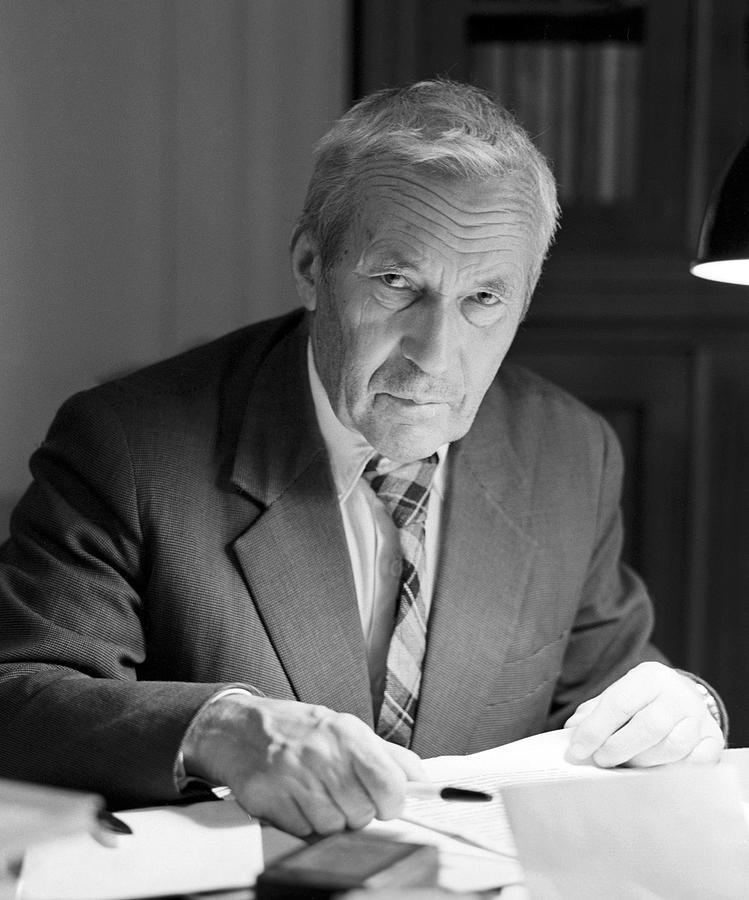
\includegraphics[width=0.7\textwidth, height=0.85\textwidth]{kolmogorov.jpeg}
          \caption{Andrey Kolmogorov (1903 - 1987)}
        \end{figure}
    \end{column}
\end{columns}
\end{frame}

%%%%%%%%%%%%%%%%%%%%%%%%%%%%%%%%%%%

\section{Stochastic Process and Time Series \parencite{brockwell2009}}

%%%%%%%%%%%%%%%%%%%%%%%%%%%%%%%%%%%

\begin{frame}
  \begin{figure}
    \centering
    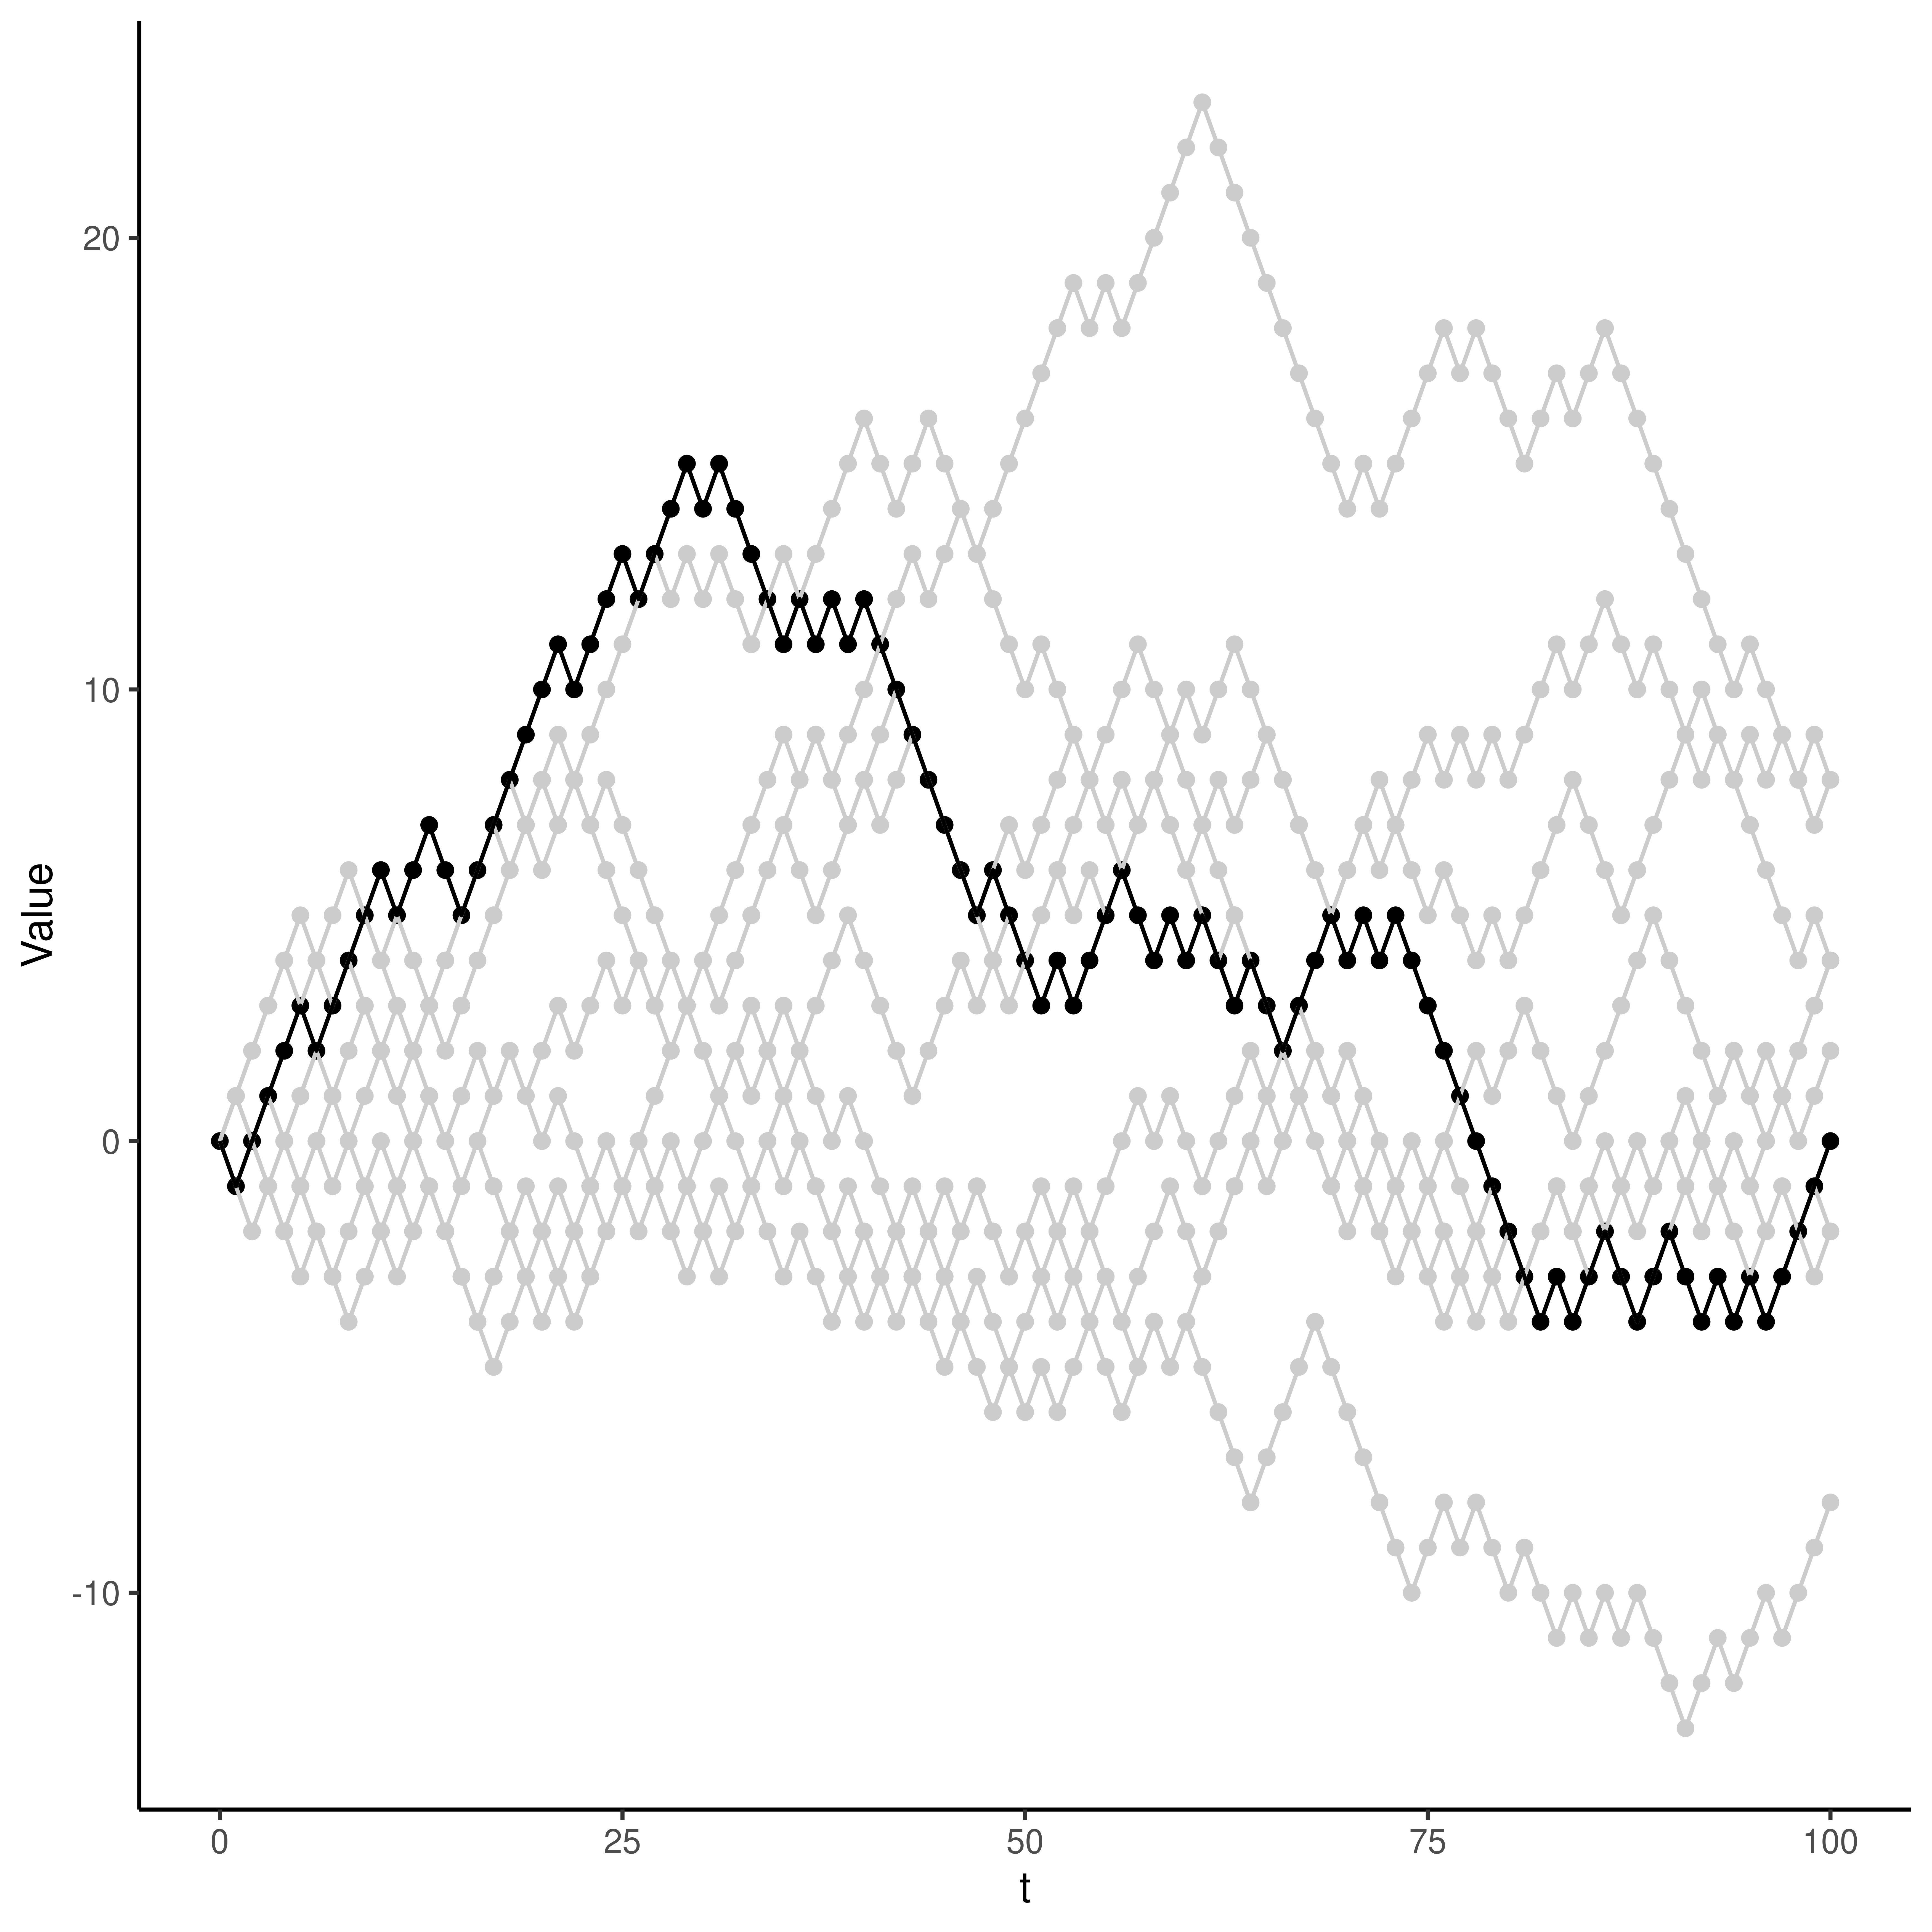
\includegraphics[width=0.7\textwidth, height=0.7\textwidth]{random_walk.jpg}
    \caption{10 realizations of the simple random walk. Here $t \in T = \{0, 1,
    \ldots, 100\}$.}
  \end{figure}
\end{frame}

%%%%%%%%%%%%%%%%%%%%%%%%%%%%%%%%%%%

\section{(Weak) Stationarity}

%%%%%%%%%%%%%%%%%%%%%%%%%%%%%%%%%%%

\begin{frame}[allowframebreaks]{References}
  \printbibliography
\end{frame}
\end{document}
